%!TEX TS-program = xelatex
%!TEX encoding = UTF-8 Unicode
\documentclass[10pt,twoside]{book}

% prevent overlapping title names and section numbering
\usepackage{tocloft}
\makeatletter
\newcommand\lahutableofcontents{%
  \if@twocolumn
    \@restonecoltrue\onecolumn
  \else
    \@restonecolfalse
  \fi
  \begin{otherlanguage}{lahu}
  \chapter*{%
    \contentsname
    \@mkboth{\MakeUppercase\contentsname}
            {\MakeUppercase\contentsname}%
  }%
  \@starttoc{tec}%
  \end{otherlanguage}
  \if@restonecol\twocolumn\fi
}
\newcommand{\addlahutoc}[2]{%
  \addcontentsline{tec}{#1}{\protect\numberline{\csname the#1\endcsname}#2}%
}
\makeatother

%%% Local Variables:
%%% mode: latex
%%% End:


\usepackage{epigraph}
\usepackage{etoolbox}
\usepackage{titlesec}

\usepackage{makeidx}
\makeindex

\usepackage{needspace}
\usepackage{fontspec}
\usepackage{xunicode} % for real tildes with \textasciitilde
\usepackage{xltxtra} % for xelatex logo
\setmainfont[Renderer=ICU,Mapping=tex-text]{Charis SIL}

\newfontfamily\tradchinesefont{BabelStone Han}
\newfontfamily\simpchinesefont{BabelStone Han}
\newcommand{\TC}[1]{{\tradchinesefont #1}}
\newcommand{\SC}[1]{{\simpchinesefont #1}}

%\usepackage{amsmath}
%\usepackage{unicode-math}
%\setmathfont[ Path = /usr/share/fonts/OTF/]{STIX2Math.otf}
%\setmathfont{STIX Two Math}

\newcommand\direct[1] {[{\DirectStyle #1}]}
\newcommand\DirectStyle {\slshape}

\usepackage{fullpage}
\usepackage{parskip}
\addtolength{\cftsecnumwidth}{10pt}
\addtolength{\cftpartnumwidth}{10pt}
%\usepackage[toc]{multitoc}
%\usepackage{supertabular,ltxtable,booktabs}
%\setcounter{LTchunksize}{600} % use more memory for fewer compiles
\usepackage{graphicx}
\usepackage[export]{adjustbox} % loads also graphicx
\usepackage{float}
% \usepackage{microtype} % only works in pdftex, which we are not using...
% \usepackage{tablefootnote}
% \usepackage{array} % use array and ragged2e for raggedright inside tables
% \usepackage[document,raggedrightboxes]{ragged2e}
% \setlength{\RaggedRightRightskip}{0pt plus 3em} % must be defined after fonts are loaded
\usepackage[yyyymmdd,hhmmss]{datetime}

\raggedbottom

\usepackage{layout}
\usepackage{fancyhdr}

% \title{Window onto a Vanished World:\\Lahu texts from Thailand in the 1960’s}
% \author{James A. Matisoff}
% \date{2019}
%\usepackage[bookmarks]{hyperref}
%\hypersetup{%
%       pdfborder={0 0 1},
%       pdfborderstyle={/S/U/W 1}, % make links underlined (instead of surrounded by red boxes)
%       pdftitle = {Window onto a Vanished World},
%       pdfauthor = {\textcopyright\ The Regents of the University of California},
%}

\makeatletter
%\patchcmd{\chapter}{\if@openright\cleardoublepage\else\clearpage\fi}{}{}{}
%\patchcmd{\chapter}{}{}{}{}
\makeatother

\usepackage{covington}
\usepackage{chngcntr}
\counterwithout{equation}{chapter}

% uniquely number examples with chapter.text
% thesection = part.chapter.section already...
% \renewcommand{\theequation}{\thesection.\arabic{equation}}
% use a single number, restart for each text
% \renewcommand{\theequation}{arabic{equation}}

\usepackage{natbib}
% references in toc
\usepackage[nottoc]{tocbibind}
\usepackage{fix-cm}
\usepackage{lettrine}
% leave this here for now, we may need it...
% \usepackage{authordate1-4}

\setlength{\headsep}{10pt}
\setlength{\headheight}{26pt}

\titleformat{\chapter}[hang]{\large\bfseries}{\thechapter}{10pt}{\large\bfseries}

\pagestyle{fancy}

\fancyhead{}

\renewcommand*{\sectionmark}[1]{ \markright{#1} }
\renewcommand*{\chaptermark}[1]{ \markboth{#1}{} }

% no 'inner' running headers for book title any more
\fancyhead[RE]{ \vspace{0.9em}}
\fancyhead[LO]{ \vspace{0.9em}}

\fancyhead[RO]{\leftmark \vspace{0.9em}}
\fancyhead[LE]{\rightmark \vspace{0.9em}}

% \renewcommand{\headrulewidth}{0.4pt}

\lfoot{}
\cfoot{\thepage}
\rfoot{}

% citation aliases
\defcitealias{STC}{STC}
\defcitealias{JAM-HPTB}{HPTB}
\defcitealias{JAM-TBRS}{TBRS}
\defcitealias{JAM-VSTB}{VSTB}

% packages for drawing trees
\usepackage{tikz}
\usepackage{tikz-qtree}

% package for enhancing lists
\usepackage[shortlabels]{enumitem}

% makes compilation really slow as we have many acronym references.
% oh well.
\usepackage[acronym,toc,nonumberlist,nopostdot,numberedsection=nameref]{glossaries}
\input{abbreviations}
\newglossaryentry{AW}{name=AW, description={Anthony T. Walker}}
\newglossaryentry{BL}{name=BL, description={Black Lahu}}
\newglossaryentry{CM}{name=CM, description={Cà-mɔ́ (chief consultant, 2nd fieldtrip)}}
\newglossaryentry{DL}{name=DL, description={The Dictionary of Lahu \citep{88}}}
\newglossaryentry{ELL}{name=ELL, description={English-Lahu Lexicon \citep{matisoff2006english}}}
\newglossaryentry{GL}{name=GL, description={The Grammar of Lahu \citep{matisoff1973grammar}}}
\newglossaryentry{H}{name=H, description={Headman (Cà-bí)}}
\newglossaryentry{JAM}{name=JAM, description={James A. Matisoff}}
\newglossaryentry{lit.}{name=lit., description={literally}}
\newglossaryentry{P}{name=P, description={Paul (Cà-lɔ̂)}}
\newglossaryentry{Si}{name=Si., description={Siamese}}
\newglossaryentry{T}{name=T, description={Teacher (Cà-bo)}}
\newglossaryentry{Ty}{name=T-y, description={Thû-yì (friend, 1st fieldtrip)}}
\newglossaryentry{RL}{name=RL, description={Red Lahu}}
\newglossaryentry{YL}{name=YL, description={Yellow Lahu}}
\newglossaryentry{Yp}{name=Yp, description={Yâ-pā-ɛ́ (chief consultant, 3rd fieldtrip)}}


\newglossary*{lexicon}{Lexicon}
\input{lexical_glossary}

% \newglossary*{baptist}{Lexicon}
% \input{blexical_glossary}

% \newglossary*{chinese}{Lexicon}
% \include{clexical_glossary}

% find a way to calculate the size of the baseline precisely
\newcommand{\quadruplehyphen}{%
\begin{tikzpicture}[baseline=-0.650ex]%
\draw [semithick] (0,-0.375ex) -- (1ex,-0.375ex);%
\draw [semithick] (0,-0.125ex) -- (1ex,-0.125ex);%
\draw [semithick] (0,0.125ex) -- (1ex,0.125ex);%
\draw [semithick] (0,0.375ex) -- (1ex,0.375ex);%
\end{tikzpicture}%
}

\makeglossaries
\begin{document}
%\layout
%\the\textwidth
%
%\the\columnwidth
%
%\the\columnsep
%\setcounter{secnumdepth}{0} % don't number sections, just chapters
\frontmatter

% we have custom title pages now... don't need maketitle
% \maketitle
\thispagestyle{empty}
\begin{center}

\vspace{4cm}
{\Large CoRSAL Occasional Publications}

\vspace{2cm}

{\Large Volume 2}

\vspace{8cm}

Series editor: Shobana Chelliah


\includegraphics[scale=0.15]{CoRSAL-Logo-BW-v03.png}

\end{center}
\clearpage{\thispagestyle{empty}\cleardoublepage}
\begin{center}
\thispagestyle{empty}
\vspace{4cm}
{\huge Window onto a Vanished World:\\\vspace{.75em}Lahu texts from Thailand in the 1960’s}

\vspace{3cm}

{\Large James A. Matisoff}
\vspace{2cm}

2022

\vspace{2cm}

Edited by

John B. Lowe

Charles Zhang

\vspace{4cm}
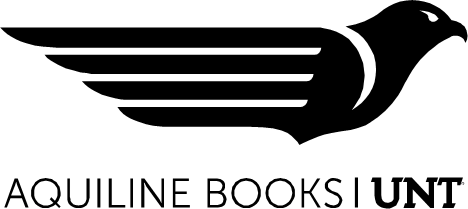
\includegraphics[scale=1]{AquilineBooksUNT.png}\\
\vspace{1cm}
An Imprint of the University of North Texas Libraries\\
\vspace{1cm}
Denton
\end{center}

\thispagestyle{empty}
\begin{center}
\vspace*{\fill}
Window to a Vanished World: Lahu Texts from Thailand in the 1960’s \\
\vspace{10em}
Published by \\
University of North Texas Libraries \\
1155 Union Circle \#305190 \\
Denton, TX  76203–5017 \\
\vspace{10em}
\copyright 2022 James A. Matisoff \\
Some rights reserved. Except where otherwise noted, this work is licensed under a Creative Commons Attribution 4.0 International License.

ISBN: 978-1-68040-[???]-[?] (paper)

DOI: https://doi.org/10.12794/sps.corsal-[???]-[?]


Requests for permission should be directed to James A. Matisoff matisoff@berkeley.edu

\vspace{10em}
\date{Compiled on \today\ at \currenttime}
\end{center}
\begin{center}
    \thispagestyle{empty}
    \vspace*{\fill}
    \Large \textit{To the Lahu people and their beautiful language}
    \vspace*{\fill}
\end{center}
\glsaddall
\clearpage{\thispagestyle{empty}\cleardoublepage}
\thispagestyle{empty}
\renewcommand{\thefootnote}{\arabic{footnote}}
\setcounter{footnote}{0}

\section*{Acknowledgments}
\sectionmark{Acknowledgments}
\addcontentsline{toc}{chapter}{Acknowledgments}
It is a pleasure to thank the many people who have made the publication
of these texts possible. First and foremost I shall always be grateful
to the Lahu villagers in Northern Thailand who welcomed me and taught me
their language in such imaginative ways during my fieldtrips in 1965--66,
1970, and 1977.

The texts I recorded during those trips were transcribed and partially
translated back in the 1960's and '70's, but processing them for
publication had to await the computer revolution. Fortunately there
was a talented cadre of computer-seasoned graduate students and
post-docs at Berkeley who were more than equal to the task. Our goals
were twofold: to produce a print version (i.e. a publication-ready PDF) of
the texts, as well as an online version (a set of static HTML pages
including links to the recordings and other metadata). Once the
transcriptions of the texts had been double-checked, Dr. J.B. Lowe
installed and configured the FLeX interlinearization program on our Mac
and imported the texts. Then we began the laborious process of providing
interlinear glosses and translations, a process
carried out over a period of several years (2013--2016), at first with
the help of Virginia Dawson and Tyler Lau.  (Following the axiom that
``If you give a man a fish you help him for one day, but if you teach
a man how to fish you help him for life'', Tyler whipped up a user's
manual for FLeX and taught me how to use it.)

Meanwhile, J.B., who had digitized the recordings from magnetic tape back in 2006,
proceeded to develop the Python scripts that would render the FLeX XML
exports into the LaTeX program, that could then generate the
final PDF. (In this effort, J.B. was assisted by Chundra
Cathcart.) The Python scripts also provided a means to match the texts
with their free translations (which we had entered as separate documents and were not included
in FLeX), to sequence the texts into sections and chapters according to
the master catalog, and to inject the necessary LaTeX code to produce
the front and back matter. My wholehearted gratitude to Dr. Lowe and the
other members of the ``team'' for their inspired work!

Finally, starting in the fall of 2017, I benefitted from Berkeley's
Undergraduate Research Apprentice Program (URAP), which made it possible
for me to retain Charles Zhang, a gifted freshman with a joint Linguistics
and Mathematics major, to finalize the process of converting the
texts and translations into LaTeX. Charles substantially amplified and improved the work,
writing code to generate glossaries and tables of contents in all three transcriptions,
updating the transducers that generated the Baptist and Chinese transcriptions, and correcting
numerous blemishes small and large. Thank you Charles for all your clever programming
and attention to details!

I'd like to thank my friend and colleague in Lahu studies, Dr. Anthony
R. Walker, for permission to republish several of his Red Lahu religious
texts.

I am most grateful to the National Science Foundation for awarding me
a grant to finish up this project (Award \#BCS1252226), which
originally ran from 9/1/13 to 2/29/16, but which was continued via a
``no-cost extension'' until August 31, 2017. I particularly want to
thank Prof.\ Joan M. Maling, program director for NSF's Social,
Behavioral, and Economic Sciences division, for her understanding and
patience during this long drawn-out process!

My sincere thanks to Paula Floro, Manager of the Berkeley Linguistics
Department, who skillfully handled the budgetary details of the NSF
grant.

My deep gratitude to Shobhana Chelliah and Mary Burke of the CoRSAL archive at
the University of North Texas
for accepting this complex manuscript as an occasional publication of
Aquiline Press, and for undertaking to ensure that the audio files associated
with the interlinear text were properly archived.

Last but not least in love, my thanks to my wife of 57 years, Susan
Kimball Matisoff, for her support every step of the way.
\clearpage{\thispagestyle{empty}\cleardoublepage}
\vspace{0.25em}

\renewcommand{\thefootnote}{\arabic{footnote}}
\setcounter{footnote}{0}

\defcitealias{matisoff1973grammar}{GL}
\defcitealias{88}{DL}
\defcitealias{matisoff2006english}{ELL}

\chapter*{Preface}
\addcontentsline{toc}{chapter}{Preface}
I certainly seem to have absorbed the Berkeley linguistics department
field worker's ethos (enunciated notably by Mary R. Haas), that if you
really want to do justice to your language, you must produce a grammar,
a dictionary, and a collection of texts. I have tried my best to do this
for Lahu. My Lahu grammar \citep[abbreviated ``GL'']{matisoff1973grammar}, appeared in 1973 (reprinted 1982); my
Lahu-English dictionary \citep[abbreviated ``DL'']{88} came out in 1988; and my English-Lahu
lexicon \citep[abbreviated ``ELL'']{matisoff2006english} was published in 2006. So this collection of texts
constitutes the third leg of the trifecta. Although these texts are the
last leg to appear, they actually have primacy, since they have formed
the basis for my grammar and dictionaries.

My study of Lahu was carried out during three major fieldtrips in
Northern Thailand (1965-66, 1970, 1977), with many shorter visits since
then, including to Lahu villages in Yunnan and Shan State.\footnote{See
\citet{matisoff2008} ``Back to my Lahu villages'' (in Chinese).} Almost all of my
work was in Christian villages, although I was fortunate enough also to
have access to the abundant material collected in animist villages by
A.R. Walker (see below).

These texts, recorded for the most part in 1965-66, over half a century
ago, reflect a vanished world: a time when the forests of Burma and
Thailand teemed with game; when slash-and-burn agricultural techniques
were universal in the hills of Southeast Asia; when animist villages
resisted the imposition of missionary Christianity, and religious
syncretism was the order of the day; a time before electricity, when
people used pine-torches to light their way at night; before young men
left the villages to seek menial work in Thai towns; before trekking
tourists came to gawk at staged ``hill-tribe'' song-and-dance shows in
Chiang Mai --- and, above all, from the linguist's point of view, a
time when the Lahu language was still vibrant in all semantic areas and
still relatively free of foreign influences.

These texts were elicited with the enthusiastic cooperation of Lahu
villagers, for whom it was a great novelty to hear the words they had
just said played back to them. Once it was made clear that I was
interested in hearing Lahu spoken in all kinds of situational
contexts, the villagers would talk over various subjects --- building a
house, the stages of cultivating a mountain field, boar-hunting, the
New Year's celebrations, gathering crabs, killing a pig for a feast,
the institution of the village headman, the government's land
policy. Then they would actually conduct rehearsals, assigning
specific roles to various people, until they felt they could discuss
the matter smoothly.  When they were satisfied, they would signal me
to turn on the tape-recorder,\footnote{It must be admitted that I
  sometimes turned on the tape-recorder before they realized it, in
  order to record still more natural
  conversation. See~\ref{sec:23},~\ref{sec:66},~\ref{sec:87}.} and
would proceed with gusto to act out little playlets on the desired
topic, often embellished with sound effects for gunshots, animal
noises, etc. Besides this kind of multi-speaker texts, many items were
also collected from individuals, including stories, songs, lectures,
and sermons. As a result of this process, which went on for many
months, the corpus comprises a wide variety of genres and registers,
including:

\emph{Discussions of serious topics} (subsistence activities, village
life and customs, relations between the Lahu and the Thai authorities)

\emph{Jokes and anecdotes}, including a well-defined genre of
\emph{bilingual jokes} (based on misunderstandings between a Black and a
Yellow Lahu, or between a Lahu and a Shan); \emph{``just-so stories''}
(etiological tales that explain why things are as they are);
\emph{trickster tales} (featuring lovable villains with
quasi-supernatural powers); myths and fairy-tales; fables and other
stories with a moral\footnote{These imaginative texts
  can be further classified to some extent in terms of the thematic
  motifs that they illustrate. See below.}

\emph{Religious texts}, including pre-Christian myths; animist prayers;
Christian sermons, hymns, Bible readings

\emph{Songs}, including traditional love poetry (which present special
difficulties); secular modern songs

For a complete list of the texts, classified by genre, see the Table of
Contents.

The true heroes of this whole enterprise were the remarkable
inhabitants of a Christian village of some twenty households about 65
km north of Chiang Mai, where the population in the 1960's consisted
of recent immigrants from Burma who had been encouraged by Baptist
missionaries to leave that country to seek a better life in
Thailand. After many adventures\footnote{See~\ref{sec:20} "How we came
  from Burma to Thailand".} they were given land in a \emph{nikhom},
or Hill Tribe Resettlement Center near Chiang Dao, where they founded
the village of Huey Tat. The two chief dignitaries of the village then
were \emph{Cà-bo}, the pastor or religious leader who conducted the
church services every Sunday (abbreviated as "T" for `teacher' in the
texts); and the newly chosen village headman, \emph{Cà-bí}
(abbreviated as "H" in the texts).\footnote{Note that many traditional
  Lahu men's names begin with the prefix \textbf{cà-}.}  Among the
younger generation, three teenagers were particularly interested and
helpful: \emph{Cà-mɔ́}, who became my chief consultant during the 1970
fieldtrip ("CM"); \emph{Thû-yì}, a fun-loving youth who died
mysteriously around 1969 (abbreviated as "T-y");\footnote{According to
  Cà-bo, Thu-yi's untimely death was due to black magic. A Northern
  Thai whom Thu-yi had beaten in a fencing match took revenge by
  making a leather mannikin which went magically into Thu-yi's belly,
  causing his death after three years of suffering.} and \emph{Yâ-pā-ɛ́
}("YP"), who was my main consultant during the 1977 fieldtrip. In
addition to the Huey Tat folks, my mainstay during the '65-'66 trip
was a city-dwelling young man called \emph{Cà-lɔ̂}, born to Lahu
parents in Shan State, who died in an epidemic when he was nine. He
was adopted into a Shan family, and stopped using Lahu regularly. At
some point he was converted by Catholic missionaries, who gave him the
name Paul (abbreviated to "P" in the texts). His Lahu had grown rusty,
but he still had the native speaker's perfect ear and accent. Paul and
I would go up to a Lahu village together for a few days, then return
to Chiang Mai to transcribe and analyze the material. Inevitably the
meanings of many words were obscure to Paul, and had to be clarified
on a following visit. After a few months of this, Paul's Lahu was
virtually indistinguishable from that of any other Lahu of his
age. After about 9 months, my own command of Lahu was such that I
would feel comfortable going to a village by myself.\footnote{Photos
  of these consultants grace the frontispieces of both GL (1973) and
  DL (1988). In many cases (especially in villages other than Huey
  Tat) I did not note who the speakers were, either because I didn't
  know their names, or because I simply forgot. At the time of this
  writing, Cà-bo, Cà-mɔ́, and Thû-yì have died, and I have lost touch
  with Cà-lɔ̂.}

It is safe to say that these texts constitute one of the largest corpora
of recorded natural speech for any minority language of the
Tibeto-Burman family. I recorded them on "primitive" reel-to-reel tape
recorders in 1965-66, under noisy field conditions, transcribing them in
longhand in some twenty field notebooks.\footnote{Speaking of
  reel-to-reel tape-recorders, I cannot resist telling the true story of
  how my recordings were nearly lost forever after I had returned safely
  to the U.S. after that first fieldtrip in 1965-66. My brother-in-law
  (also named Jim) picked us up from the SFO airport in his little
  Volkswagen bug. There were four people in the car, so some of our
  baggage (including my tapes and fieldnotes) had to be crammed into the
  roofrack. Jim had neglected to bring bungee cords or twine, so we
  headed onto the freeway hoping for the best. Unfortunately the
  suitcases soon flew off the roof onto the highway, spewing the reels
  of tape all over. Let us draw the curtain of charity over the rest of
  this scene, although there was a happy ending. The martyred tapes were
  wrapped in a quilt and rescued from oncoming traffic, and the
  magicians in the Berkeley Language Lab were able to restore almost all
  of them, although with some loss of their already not wonderful
  fidelity.} At the conclusion of this fieldtrip, I began my first
teaching job, at Columbia, where I began the task of translating the
texts, managing to complete drafts of 34 of them before other duties
made me put the job on hold. Nevertheless, these texts, both translated
and untranslated, formed the basis for my Lahu grammar (1973/1982), as
well as a good part of the material for my Lahu dictionary (1988).

Meanwhile another research project which was to consume most of my
attention for over a quarter century was getting under way: the
\emph{Sino-Tibetan Etymological Dictionary and Thesaurus} project
(STEDT), funded jointly at Berkeley by the National Science Foundation
and the National Endowment for the Humanities from 1987-2014. This of
course was the era when computers were revolutionizing the academic
world, and I was fortunate in having a brilliant computer-savvy staff
of graduate students to help. Foremost among these was John B. Lowe
("J.B."), who not only designed the structure of the STEDT database,
but also contributed to liberating my Lahu texts from the back burner
by digitizing the original magnetic tape recordings from 1965-66, a
job he carried out at the Berkeley Language Center in
2006.\footnote{As a pilot project in the processing of the texts, we
  were able to invite Michel Jacobson, a computer specialist at the
  LACITO project in Paris (\emph{Langues et Civilisations à Tradition
    Orale}, a branch of the Centre National de la Recherche
  Scientifique) to spend a month at Berkeley in \emph{\textbf{20XYZ}}
  to produce time-aligned interlinear texts using the LACITO Archive
  tools. As it turned out, only a single short text ("How we came from
  Burma to Thailand", \ref{sec:20}.) was processed during Michel's
  stay in Berkeley, although it was a valuable experience to see what
  would be involved in preparing the texts for publication with the
  software then available.}

There matters stood with the texts until 2009, when I made the
acquaintance of a Burmese Lahu graduate student in linguistics at Payap
University in Chiang Mai, Thailand, named Aaron ``Maung Maung'' Tun, who
has both an impressive linguistic acumen and a strong desire to make the
results of my work more accessible to the Lahu people. Maung Maung was
able to spend two and a half months as a Visiting Scholar at Berkeley in
the spring of 2011. During his stay he checked over all my
transcriptions by comparing them to the sound-files, and also helped
J.B. to segment the digitized files (which contained the contents of
whole tapes) into separate files corresponding to the texts they
represented. Maung Maung (a nickname meaning ``younger brother'' in
Burmese) was also able to clarify certain incomprehensible passages,
e.g. when several people talked at once.

These developments were so encouraging that I was motivated to apply for
another NSF grant to prepare all the texts for publication. This
application was happily successful, and the project was funded from
Sept. 2013 until Feb. 2016, with a ``no-cost extension'' assuring its
continuation until mid-2017.\footnote{For more details about the
  personnel involved during this new grant, please see the
  \emph{Acknowledgments}.}

The present volume includes only about 139 texts out of some 216 items
recorded. Reasons for non-inclusion include the following:

\begin{itemize}
\item The item was musical, either instrumental (jewsharp, gourdflute)
  or choral (hymns sung in harmony in church). However, as a sample
  nine of the latter have been included.\footnote{See "Christian
    hymns and Bible readings", chapter~\ref{chapter:Christian hymns
      and Bible readings} in the Table of Contents.}

\item
  The item was too badly recorded for comprehension, or so badly told
  that the point was unclear.
  
\item The item was in non-standard Black Lahu (i.e. Red Lahu or Lahu
  Shehleh), so that the meanings of many lexical items were not clear
  to me or my consultants. (Many texts in Yellow Lahu have been
  included, however, as have Walker's animist texts in Red
  Lahu.\footnote{Most of the Yellow Lahu texts appear in the section
    on \emph{Bilingual humor}, chapter~\ref{chapter:Bilingual humor}. Several of Walker's Red Lahu texts
    are to be found in chapter~\ref{chapter:Traditional theo - animism}, \emph{Traditional
      ``theo - animism''}.}
  
\item
  The item was in archaic poetic language that consultants were
  unfamiliar with. This is the case with many of the lovesongs I recorded.
  Some of the more transparent ones are included in this volume.\footnote{See
    "Traditional songs", chapter~\ref{chapter:Traditional songs}. These lovesongs were already
    fading from use in the 1960's. They were once elaborate antiphonal
    performances, men alternating with women, using a rich store of set
    expressions, with much repetition. The flavor of these beautiful texts
    can be gathered from the long translations in \citet[][pp. 151-174]{y13}.}
\end{itemize}

The presentation of the texts follows a certain format. Each one first
appears as a three-line complex, with the top line containing the more
or less verbatim Lahu, the middle line providing a form-class
designation for each word,\footnote{See page~\pageref{acronym} for
  an alphabetical list of these symbols. Similar lists appear in my
  Lahu Grammar \citep[pp. xxviii- xxxvii]{matisoff1973grammar}, and
  Dictionary \citep[pp. xxi-xxiv]{88}. In Haudricourt's otherwise
  highly positive review of the Grammar \citep{h74}, he ruefully
  referred to its form-class list as ``hélas, de dix pages!''}  and the
bottom line giving a concise English gloss appropriate to the
particular context. These interlinear glosses were generated by the
tricky but ingenious FLEX program (see below). After the word-by-word
translation comes the free translation, accompanied by explanatory
footnotes.

In the printed version of this book the Lahu texts are given in my own
transcription.\footnote{For a threnody of belated regrets for my
  phonemically accurate but rather difficult transcription, see
  \citet{matisoff2014}.} In the electronic version, they are also presented
in the Baptist and Chinese orthographies. Equivalency charts of these
three systems (as well as the little-used Catholic one) are given in
the introduction to \citet[pp.14-28]{88}. My transcription of words in
the divergent Yellow Lahu dialect is rather
impressionistic.\footnote{See \citet{matisoff1969lahu} for details.}

A few minor transcriptional points:

\begin{itemize}

\item
  \emph{Vowel nasalization} in Lahu is always optional, occurring
  either in loanwords where the donor language had a final nasal, or
  in native syllables beginning with \textbf{h-} or zero-initial by a
  phenomenon I have dubbed ``rhinoglottophilia".\footnote{See
    \citet{m75}.} In a dictionary this variability can be indicated by
  parentheses, e.g. \textbf{ɔ̀-bo(n)} `grace', \textbf{ká(n) }`work',
  \textbf{hɔ́(n) }`fragrant', \textbf{hɔ(n) }`elephant', \textbf{ɔ̂(n)}
    `four'. In the texts I tried to respect the particular variant
  used by the speaker on that occasion. Writing the \textbf{-n} is
  sometimes useful in disambiguating homophones, e.g. \textbf{ɔ̀-yâ}
  `son/child' / \textbf{ɔ̀-yân} `time' (\textless{} Tai).

\item
  \emph{Interjections }are usually pronounced with exaggerated or
  drawled intonation. This is indicated by writing them with double
  vowels, e.g.  \textbf{âa}, \textbf{ôo}, \textbf{pòthôo},\textbf{
    alôo}.

\item
  \emph{Hyphenization} Compound constituents are written with
  hyphens between the syllables. In \emph{DL:51-52} I explained my
  system of multiple hyphens that indicate how polysyllabic compounds
  are to be segmented, e.g. \textbf{ɔ́-qā} `water buffalo',
  \textbf{ɔ́-qā=qhɛ̂} `buffalo dung', \textbf{ɔ́-qā=qhɛ̂≡phôʔ} `pile of
  %% change to quadruple
  buffalo dung', \textbf{ɔ́-qā=qhɛ̂≡phôʔ≡-ló} `big pile of buffalo
  dung'.\footnote{In \emph{DL} I connected the bound nominal morpheme
    ló(n) `big; great' to the preceding noun by a hyphen, but in the
    texts I have omitted the hyphen for convenience's sake. To have
    left the hyphen in would have been to force new unitary glosses
    like `big X', where X stands for any semantically appropriate
    noun.} As I bravely said, ``I do not flinch from using triple or
  quadruple hyphens as necessary.'' In the present volume, however,
  there is never any need to go beyond single hyphens.

\end{itemize}

At first I felt obliged to transcribe the texts verbatim, to the point
where I was including all the hesitations, false starts, and repairs
that the speakers made. However, this soon came to feel pedantic, so I
mostly stopped doing it. In fact I have lightly edited many of the
texts for clarity's sake.\footnote{I accorded the same treatment to my
  own previously published texts illustrating the genre of bilingual
  humor (see \citet{matisoff1969lahu} and section
  \ref{chapter:Bilingual humor}, as well as the six animist religious
    texts recorded by Anthony Walker that have been included in
    section~\ref{chapter:Traditional theo - animism}). Needless to
    say I received Anthony's permission before editing his
    translations.}

In the free translations I have attempted to stick as closely as
possible to the Lahu while coming up with readable and natural English
versions. This has been no easy task in view of the vast differences in
structure and information-packaging strategies between Lahu and English.
The interlinear glossing has presented its own set of
challenges,\footnote{As mentioned above, the interlinear glossing was
  done using the FLEX program developed by the Summer Institute of
  Linguistics (SIL), which, despite its many virtues, is rather buggy
  and delicate to use.} largely due to the pervasive problems of
polysemy and homophony.

In a phonologically eroded language like Lahu, with no syllable-final
consonants or initial consonant clusters, homophonous morphemes abound,
where the initials, vowels, and tones are all identical. This has made
it impossible totally to automate the glossing process. A few examples:

\textbf{qɔ̂} `nine'; `coffin'; `to hoe'; `empty/hollow'; `loose' (DL
251-253)

\textbf{qhɔ} `mountain'; `inside'; be open (of a wound); `coiled up'
(DL 299-304)

\textbf{thɔ̂} `touch'; `pine tree'; `also/even'; `calendrical animal' (DL
691-692)

\textbf{mâ} `many'; `not' (DL 965-975)

\textbf{šī} `know'; `lead/conduct'; `choke'; `sharpen'; `round object'
(DL 1185-1188)

\textbf{šɛ̄} `smear on'; `cymbals'; `pay back money'; `liver'; `body';
`fingernail'; `three'

\textbf{là} `tea'; `come'; `million' (DL 1351-1352)

\textbf{lâ} `tiger'; `non-3p benefaction'; `yes/no question' (DL
1345-1347)

In the early stages of interlinearization we dealt with polysemy by
using alternative interlinear glosses, as in a dictionary, with the
alternatives separated by a slash, e.g., `begin/start', `flee/run away',
`persuasive/urging', `delicious/tasty', etc. This soon seemed messy,
however, so I went through all the texts again, giving single glosses
for each item as it appeared in its particular context. It was
especially important to distinguish between the meaning a verb has when
it functions as the main verb in its VP as opposed to the ``bleached'' or
``grammaticalized'' meaning it acquires when it appears as an auxiliary or
``versatile'' verb, e.g. \textbf{chɛ̂} `live/dwell' (main verb) vs.
`progressive/continuative' (versatile verb); \textbf{g̈a} `get/obtain'
(main verb) vs. ``manage to; able to; get to'' (versatile verb);
\textbf{tɔ̂ʔ} `emerge' (as main verb) vs. `outward' (versatile verb).

Sometimes a whole phrase is glossed as a single word, even though no
hyphen appears between its syllables, e.g. \textbf{tê yân thâ} `when'.
At other times the identical phrase might be broken down into
constituents, each glossed separately and with a separate form-class
designation: \textbf{tê (}Num) `one/a' + \textbf{yân (}Clf) `time' +
\textbf{thâ (}P\textsubscript{univ}) `time that', lit. "at a time that".

It is difficult but vital to give precise glosses to functors in
particular contexts. Thus the thousands of occurrences of the most
important particle in the language, \textbf{ve}, had to be glossed in
three different ways, either as `nominalizer' or `relativizer' or
`genitivizer'.\footnote{See \citet{matisoff1972}.} The particular context
dictated whether the verb-particle \textbf{tā} was to be glossed as
`durative' or `perfective'; whether the verb-particle \textbf{ò} was
better glossed as `completed action' or `change of state'; whether the
verb-particle \textbf{šē} functioned as `inchoative' or as a `marker of
regret'; whether the versatile verb \textbf{chɛ̂} should be called
`progressive' or `continuative'; whether the final unrestricted particle
\textbf{mɛ̄} was `urging' or `persuasive' in a particular sentence.

Lahu is what has been quaintly called a ``pro-drop''
language,\footnote{I call this term ``quaint'' since it implies that
  the pronouns were once there but have been dropped. A better way to
  look at it is that the overt presence of pronouns is optional in the
  first place.} i.e. a language where pronouns are often omitted when
the situation seems clear to the speaker and listener. This often
makes it hard to see what is happening to whom in connected
narratives. Compounding the problem are the facts that Lahu has no
gender distinction in third-person pronouns, no case-marking for
pronouns (beyond a sparingly used accusative particle, \textbf{thàʔ}),
and no honorific pronouns (unlike literary languages like Thai,
Burmese, or Khmer).\footnote{A title rather than a pronoun may be used
  when talking to or about a respected person, e.g. \textbf{qhâʔ-sɛ}
  `headman', \textbf{šālàʔ-ló} `great teacher', etc. } Thus the 3rd
person pronoun \textbf{yɔ̂ }may be translated as \emph{he, him, she,
  her, his, hers, He, Him, His}.\footnote{Pronouns often occur
  directly before a noun with genitive meaning, hence the possible
  glosses `his' or `her'.  When the pronoun refers to a deity I spell
  the translation with a capital letter. Cf. the five different
  characters now used in Mandarin to differentiate the various
  possible referents of the same 3rd person pronoun
  \textbf{tā}: 他 `he/she', 她 `she', 它 `it' (inanimate), 祂`He
  (deity)', 牠 `he/she (animal)'.} Similarly, the remote 3rd person
pronoun \textbf{šu }has a large number of possible
translations: he, non-Lahu, other people,
others, others', she, somebody, somebody else, somebody else's,
somebody's, the other guy, their, them, they.

Equally challenging is the lack of a morphological plural marker in
Lahu, so that a word like \textbf{chɔ} `person' must be translated
either as `person' or `people' according to context.

In several cases I recorded the same story as told by different people.
Since it is useful to see individual variations in story-telling
technique, both versions have been included. See ``The smoker and the
non-smoker dispute a pipe''~\ref{sec:121}; ``In unity there is strength'' \ref{sec:27};
``The three lazy men and the princess''~\ref{sec:83}; ``The trader and the
widow's balls/daughter''~\ref{sec:33}.

Many of the stories illustrate universal fairy-tale motifs (e.g. a
wicked older sibling and a good younger one).\footnote{A classic index
  of motifs in folk literature is Thompson 1955-58.} Widows and
orphans frequently appear, as do fathers-in-law and their sons-in-law
(a rather fraught relationship among the Lahu, since a new son-in-law
traditionally had to work for several years in his father-in-law's
fields before setting up his own household). Trickster stories are a
well-established genre, with Chinese traders often serving as foils
for the trickster's shenanigans. Often someone with a physical problem
(especially being blind or crippled) is miraculously cured. Sometimes
a physical deformity actually proves to be a saving grace (see ``The
fingerless lord'', \ref{sec:94}). Some of the stories seem to go back
to Aesop (``The blind men and the elephant'',~\ref{sec:30}; ``In unity
there is strength'',~\ref{sec:27}; ``The boastful cock and the
hawk'',~\ref{129}), perhaps via the Indian fabulist Pilpay (or
Bidpai).\footnote{Pilpay was a collector of Sanskrit animal fables who
  flourished before A.D. 500, and whose work entered European
  literature through an Arabic version (ca. A.D. 750). The 17th
  century French fabulist La Fontaine seems to have been familiar with
  his work.}


\protect\hypertarget{anchor}{}{}The texts reflect a wide variety of
styles, ranging from highly colloquial conversations to serious
sermons in church. Despite the fact that most of the texts were
recorded in Christian villages, there is nothing Christian about the
content of many of them, e.g. the racy cycle of Trickster stories
(\ref{sec:38}, \ref{sec:39}, \ref{sec:92}, \ref{sec:95},
\ref{sec:40}), or the anecdotes about farting contests
(\ref{sec:34}). It should be said that the Lahu are anything but
prudish about matters sexual or scatological. There are no "dirty
words" in the language, but only one word for each body part and
physical activity, usable matter-of-factly in any context.

A number of the texts have already been published elsewhere:

For the anecdotes involving bilingual humor~\ref{chapter:Bilingual humor}, see Matisoff 1969

\begin{itemize}
\item ''The little crabs who walked zigzag''~\ref{sec:96} was
  translated in Matisoff 1973b.

\item ''Trickster and the village women''~\ref{sec:40} appeared in
  Matisoff 1979.

\item ''Praying for game''~\ref{sec:207} was published in Matisoff
  1979.

\item ''The boastful cock and the hawk''~\ref{sec:129} appeared in
  both English and Chinese in Matisoff 2002

\item For the references to Anthony Walker's six animist texts
  included in~\ref{chapter:Traditional theo - animism}, see the
  \emph{Bibliography}.

A few words about cultural change and linguistic endangerment might be
appropriate here. It seems to me that the whole notion of endangerment
seems to require some refinement. The Lahu language is not in immediate
danger of extinction, largely due to the fact that Lahu villages are
dispersed across several countries. The Lahu population has been
increasing, and the language is still spoken by people of all ages. On
the other hand, the language has been coming under ever-increasing
pressure from the coterritorial prestige languages with which it is in
contact: Mandarin in Yunnan, Shan and Burmese in Myanmar, Northern Thai,
Standard Thai, Lao, and Vietnamese. Loanwords from these majority
languages are flooding into the Lahu vocabulary. While some cultural
practices remain more or less vital, such as the New Rice Festival in
the autumn and the two-week long New Year's celebrations, the effects of
globalization and homogenization are everywhere. There are now shortwave
radios, TV's, and CD players in every village. Traditional story-telling
around the fire is a thing of the past. Whole areas of the Lahu lexicon
have virtually disappeared from the vocabularies of the last several
generations of speakers: the endearments of traditional love poetry;
animist prayers to the spirits; swidden (mountain-field) agricultural
terms; flora and fauna names; weaving terminology; hunting terms, and so
on.

The whole notion of endangerment seems to require some refinement. The
Lahu language is not in immediate danger of extinction, largely due to
the fact that Lahu villages are dispersed across several countries. The
Lahu population has been increasing, and the language is still spoken by
people of all ages. On the other hand, the language has been coming
under ever-increasing pressure from the coterritorial prestige languages
with which it is in contact: Mandarin in Yunnan, Shan and Burmese in
Myanmar, Northern Thai, Standard Thai, Lao, and Vietnamese. Loanwords
from these majority languages are flooding into the Lahu vocabulary.
While some cultural practices remain more or less vital, such as the New
Rice Festival in the autumn and the two-week long New Year's
celebrations, the effects of globalization and homogenization are
everywhere. There are now shortwave radios, TV's, and CD players in
every village. Traditional story-telling around the fire is a thing of
the past. Whole areas of the Lahu lexicon have virtually disappeared
from the vocabularies of the last several generations of speakers: the
endearments of traditional love poetry; animist prayers to the spirits;
swidden (mountain-field) agricultural terms; flora and fauna names;
weaving terminology; hunting terms, and so on.

In all the countries where Lahu is spoken, it is not a majority
language, and is in fact only one of a large number of minority
languages. It is still the first language of most Lahu children, but
educational materials in Lahu hardly exist beyond the second or third
grade level. After that the only available schooling is in the majority
language. Intermarriage between Lahu and other Tibeto-Burman minority
groups (e.g. Jingpho, Lisu), or between Lahu and majority-group members,
is still relatively rare, but seems now to be on the increase. There are
a certain number of CD's in Lahu produced in Burma or China, and
available in some Lahu villages in Thailand.

\emph{}

Lahu traditional culture has been encroached upon from two directions:
from coterritorial majority cultures (Chinese, Burmese, Tai,
Vietnamese), and from the Western world via evangelical Christianity.
Misguided strictures against swidden rice cultivation (which is
frequently referred to as ``slash-and-burn'' agriculture, but actually
has numerous ecological benefits when practiced correctly), along with
governmental prohibitions against opium cultivation, have revolutionized
traditional Lahu agriculture. Tea and coffee plantations and fruit
orchards, owned by Thai or Chinese businessmen, now offer employment
opportunities for young people, who have grown accustomed to the
formerly alien notion of working for a salary.

Contact with the money economy has brought with it prostitution and
AIDS,

consumerism, and hard drug use, with amphetamines replacing the
comparatively benign (and often medically useful) opium.

Virtually all the Lahu in Thailand have now been converted to
Christianity by American, Australian, and European missionaries, both
Baptist and Catholic. In the 1960's most of Thailand's 30,000 Lahu were
still animistic in religion, with some Buddhist influences.

As mentioned above, my friend and colleague, the British anthropologist
Dr. Anthony R. Walker, spent four consecutive years in an animist
village in Northern Thailand in the late 1960's, and collected a
prodigious number of Red Lahu animist religious texts, which he has
gradually published in journals all over the world (although they have
not yet been assembled in a single volume). The specialized, archaic
vocabulary items in all these texts were incorporated into my dictionary
in the 1970's. There have been other notable recordings of traditional
religious texts in Loloish languages, notably Ma Xueliang (1949) for
Luquan Lolo/Yi; and Inga-Lill Hansson (in prep.) for Akha, opening up
a tempting field for future comparative work in this area.

It is my hope that these texts will bring pleasure to the Lahu people
themselves, as well as to anyone interested in Southeast Asian
languages and culture.



%%%% (setq bibtex-completion-bibliography '("~/Lahu/contents/interlinear/stedtreferences.bib"))
\clearpage{\thispagestyle{empty}}
\part*{Symbols and Abbreviations}
\addcontentsline{toc}{chapter}{Symbols and Abbreviations}
\setglossarysection{section}
\printglossary[type=\acronymtype,title=Form Class Abbreviations]
\printglossary[title=Miscellaneous Abbreviations]
% \thispagestyle{empty}
\cleardoublepage

%\pdfbookmark[0]{Table of Contents}{TOC}
\tableofcontents
\lahutableofcontents
% \baptisttableofcontents
% \chinesetableofcontents


\mainmatter
%\pdfbookmark[0]{Window onto a Vanished World}{TOC}

% insert includes here

\cleardoublepage
\backmatter
\setglossarysection{chapter}
\addcontentsline{lahutable}{chapter}{dîʔšōnēli-ɛ́}
\printglossary[type=lexicon, title={Glossary, phonemic transcription}, style={long}]
%\addcontentsline{baptisttable}{chapter}{diˆshon\protect\underline{\protect\phantom{x}}e\protect\underline{\protect\phantom{x}}li-eh¯}
%\printglossary[type=baptist, title={Glossary, in Baptist transcription}, style={long}, sort={letter}]
%\addcontentsline{chinesetable}{chapter}{ditshofnefli-ieq}
%\printglossary[type=chinese, title={Glossary, in Chinese transcription}, style={long}, sort={letter}]
\glsunsetall

\cleardoublepage
\bibliographystyle{authordate1}
\renewcommand{\bibname}{References}
\addcontentsline{lahutable}{chapter}{Lâhū-khɔ̂ cá dàʔ ve lìʔ-qôʔ}
%\addcontentsline{baptisttable}{chapter}{Laˇhu\protect\underline{\protect\phantom{x}}-hkawˇ ca¯ da‸ ve li‸-k’oˆ}
%\addcontentsline{chinesetable}{chapter}{Ladhuf-khawd caq dar ve lir-qot}
\nocite{*}
\bibliography{stedtreferences}
\fancyhead[LE]{\large{References} \vspace{0.5em}}
\fancyhead[RO]{\large{References} \vspace{0.5em}}

\end{document}
